\documentclass[10pt,twocolumn]{article}
% Shared two-column preamble for the three research papers.
% Use with: \documentclass[10pt,twocolumn]{article}
% Then in main.tex: % Shared two-column preamble for the three research papers.
% Use with: \documentclass[10pt,twocolumn]{article}
% Then in main.tex: % Shared two-column preamble for the three research papers.
% Use with: \documentclass[10pt,twocolumn]{article}
% Then in main.tex: \input{../../shared/latex/twocolumn_preamble.tex}

\usepackage[margin=0.75in]{geometry}
\usepackage[utf8]{inputenc}
\usepackage[T1]{fontenc}
\usepackage{lmodern}
\usepackage{microtype}
\usepackage{amsmath,amssymb,amsthm}
\usepackage{graphicx}
\usepackage{booktabs}
\usepackage{caption}
\usepackage{subcaption}
\usepackage{hyperref}
\usepackage{url}
\usepackage{xcolor}
\usepackage{algorithm}
\usepackage{algorithmic}
\usepackage{multirow}
\usepackage{titlesec}
\usepackage{authblk}

\hypersetup{colorlinks=true,linkcolor=blue!50!black,citecolor=blue!50!black,urlcolor=blue!50!black}

\titleformat{\section}{\normalfont\large\bfseries}{\thesection}{0.6em}{}
\titleformat{\subsection}{\normalfont\bfseries}{\thesubsection}{0.5em}{}

\captionsetup{font=small,labelfont=bf,skip=4pt}
\setlength{\columnsep}{0.25in}
\setlength{\parskip}{2pt}

\newtheorem{theorem}{Theorem}
\newtheorem{proposition}[theorem]{Proposition}
\newtheorem{definition}[theorem]{Definition}


\usepackage[margin=0.75in]{geometry}
\usepackage[utf8]{inputenc}
\usepackage[T1]{fontenc}
\usepackage{lmodern}
\usepackage{microtype}
\usepackage{amsmath,amssymb,amsthm}
\usepackage{graphicx}
\usepackage{booktabs}
\usepackage{caption}
\usepackage{subcaption}
\usepackage{hyperref}
\usepackage{url}
\usepackage{xcolor}
\usepackage{algorithm}
\usepackage{algorithmic}
\usepackage{multirow}
\usepackage{titlesec}
\usepackage{authblk}

\hypersetup{colorlinks=true,linkcolor=blue!50!black,citecolor=blue!50!black,urlcolor=blue!50!black}

\titleformat{\section}{\normalfont\large\bfseries}{\thesection}{0.6em}{}
\titleformat{\subsection}{\normalfont\bfseries}{\thesubsection}{0.5em}{}

\captionsetup{font=small,labelfont=bf,skip=4pt}
\setlength{\columnsep}{0.25in}
\setlength{\parskip}{2pt}

\newtheorem{theorem}{Theorem}
\newtheorem{proposition}[theorem]{Proposition}
\newtheorem{definition}[theorem]{Definition}


\usepackage[margin=0.75in]{geometry}
\usepackage[utf8]{inputenc}
\usepackage[T1]{fontenc}
\usepackage{lmodern}
\usepackage{microtype}
\usepackage{amsmath,amssymb,amsthm}
\usepackage{graphicx}
\usepackage{booktabs}
\usepackage{caption}
\usepackage{subcaption}
\usepackage{hyperref}
\usepackage{url}
\usepackage{xcolor}
\usepackage{algorithm}
\usepackage{algorithmic}
\usepackage{multirow}
\usepackage{titlesec}
\usepackage{authblk}

\hypersetup{colorlinks=true,linkcolor=blue!50!black,citecolor=blue!50!black,urlcolor=blue!50!black}

\titleformat{\section}{\normalfont\large\bfseries}{\thesection}{0.6em}{}
\titleformat{\subsection}{\normalfont\bfseries}{\thesubsection}{0.5em}{}

\captionsetup{font=small,labelfont=bf,skip=4pt}
\setlength{\columnsep}{0.25in}
\setlength{\parskip}{2pt}

\newtheorem{theorem}{Theorem}
\newtheorem{proposition}[theorem]{Proposition}
\newtheorem{definition}[theorem]{Definition}

\newcommand{\qwenZeroFivebBaselineAcc}{0.688}
\newcommand{\qwenZeroFivebAccBitsFour}{0.312}
\newcommand{\qwenZeroFivebAccBitsTwo}{0.000}
\newcommand{\qwenZeroFivebMSEBitsFour}{7.4160}
\newcommand{\qwenZeroFivebMSEBitsTwo}{13.7376}
\newcommand{\qwenZeroFivebSensAttnDeltaAcc}{-0.062}
\newcommand{\qwenZeroFivebSensAttnMSE}{1.7806}
\newcommand{\qwenZeroFivebSensMlpDeltaAcc}{-0.375}
\newcommand{\qwenZeroFivebSensMlpMSE}{4.0926}


\title{Bit-Width Scaling Laws for Mathematical Reasoning in Small Language Models}
\author[1]{Luis Benvenuto}
\affil[1]{Independent Research}
\date{June 16, 2026}

\begin{document}
\twocolumn[\maketitle
\begin{@twocolumnfalse}
\begin{abstract}
\noindent We study how post-training quantization of the weights of a small
autoregressive language model affects its ability to approximate
elementary mathematical functions. A dependency-free per-channel symmetric
quantizer is applied at bit-widths $\{32, 16, 8, 4, 2\}$, where 2-bit
corresponds to a ternary BitNet-style approximation. On the open-weight
Qwen2.5-0.5B model evaluated on a synthetic arithmetic benchmark, we observe
the expected monotonic degradation: logit MSE versus the FP32 reference
spans many orders of magnitude across the sweep. Layer-wise submodule
sensitivity reveals that attention and feed-forward weights contribute
asymmetrically to the residual error. The pipeline is configuration-driven
and rescales to GSM8K, the Hendrycks MATH benchmark, and 7B-parameter
mathematical models behind a GPU configuration.
\end{abstract}
\vspace{1em}
\end{@twocolumnfalse}]

\section{Introduction}
Quantization is now the dominant technique for deploying large language
models on commodity hardware. Yet whilst memory and latency benefits are
well-understood, the question of \emph{which capabilities degrade first}
under aggressive precision reduction remains open. Mathematical reasoning
is a natural stress test: arithmetic and symbolic problems require many
sequential non-linear approximations and amplify errors quickly.

\paragraph{Question.} How does the residual error in non-linear function
approximation by a small open-weight language model scale with the
bit-width of its parameters, and which submodules---attention or
feed-forward---contribute most to that error?

\paragraph{Contributions.} (i) A dependency-free per-channel symmetric
quantizer covering FP32, FP16, INT8, INT4, and ternary (1.58-bit) regimes.
(ii) A reproducible evaluation pipeline combining a synthetic arithmetic
benchmark with optional GSM8K loading. (iii) A submodule-sensitivity test
isolating attention from feed-forward contributions to logit error. (iv) An
end-to-end paper whose numbers and figures are regenerated from raw results
on each run; the same code rescales to TinyLlama-1.1B and Qwen2.5-Math-7B
via the GPU configuration.

\section{Related Work}

\paragraph{Post-training quantization (PTQ).}
GPTQ~\cite{frantar2022gptq} and AWQ~\cite{lin2023awq} achieve nearly
loss-less INT4 weights via second-order error correction and
activation-aware scaling. SmoothQuant~\cite{xiao2022smoothquant} migrates
activation outliers into the weights. We deliberately use a simpler
per-channel symmetric quantizer to establish a clear lower bound on the
quality--bit-width trade-off; better quantizers are a strict improvement,
not a contradiction.

\paragraph{Ternary and BitNet.} BitNet~\cite{wang2023bitnet} demonstrates
that training from scratch with ternary weights $\{-1,0,+1\}$ can match
FP16 baselines at sufficient scale. Our 2-bit setting is post-training and
is best interpreted as a stress test, not a recipe.

\paragraph{Mathematical capabilities of LLMs.}
GSM8K~\cite{cobbe2021gsm8k} and the Hendrycks MATH benchmark
\cite{hendrycks2021math} are the canonical evaluations. Our local
configuration uses synthetic arithmetic problems so that the pipeline runs
deterministically without network access; the GPU configuration substitutes
GSM8K and MATH subsets.

\section{Methodology}

\subsection{Quantizer}
Let $W \in \mathbb{R}^{n_{\text{out}} \times n_{\text{in}}}$ be the weight
of a linear layer. We use the following per-row symmetric quantizer:
\begin{itemize}
\item \textbf{32-bit:} identity.
\item \textbf{16-bit:} cast to FP16, round-trip back to working dtype.
\item \textbf{8 / 4-bit:} symmetric per-row scale
$s_i = \max_j |W_{ij}| / q_{\max}$, with
$q_{\max}\in\{127,7\}$ and the quantized weight
$W'_{ij} = s_i \cdot \mathrm{clip}\bigl(\mathrm{round}(W_{ij}/s_i),\,\pm q_{\max}\bigr)$.
\item \textbf{2-bit (ternary):} per-row threshold $\tau_i = 0.7\,\bar{|W|}_i$,
where $\bar{|W|}_i$ is the row's mean absolute value.
Weights below the threshold are zeroed; surviving weights take values
$\pm s_i$, where $s_i$ is the mean magnitude of surviving weights.
This is a deterministic, dependency-free approximation of BitNet's
ternary regime.
\end{itemize}

\subsection{Logit divergence}
For each problem we record the model's last-token logits under FP32 and
under each quantization regime, and compute
$\mathrm{MSE} = \mathbb{E}\bigl[(\ell^{\mathrm{ref}} - \ell^{q})^2\bigr]$
and the forward KL divergence
$\mathrm{KL}(p \,\|\, q)$ between the corresponding softmax distributions.
MSE measures raw drift; KL is sensitive to the decisive directions of the
distribution.

\subsection{Submodule sensitivity}
We isolate attention vs.\ feed-forward error contributions by applying
quantization \emph{only} to layers whose module path contains
$\{\texttt{attn}, \texttt{attention}, \texttt{self\_attn}\}$ or
$\{\texttt{mlp}, \texttt{ffn}, \texttt{feed\_forward}, \texttt{fc}\}$
respectively, holding the complement at FP32.
The bit-width used for this experiment is 4, the regime where the global
sweep shows the steepest accuracy degradation.

\section{Experiments}

\paragraph{Model.}
Qwen2.5-0.5B (the open-weight 494M-parameter Qwen model). The GPU
configuration switches to TinyLlama-1.1B-Chat-v1.0 and Qwen2.5-Math-7B
without code changes.

\paragraph{Benchmark.}
A deterministic synthetic arithmetic benchmark of 80 items spanning
addition, subtraction and multiplication with operands sampled uniformly
from $\{1,\dots,100\}$, plus optional GSM8K subset behind
\texttt{gpu\_full.yaml}. Accuracy is judged by string-matching the first
integer in the model's greedy completion.

\paragraph{Procedure.}
For each bit-width $b \in \{32, 16, 8, 4, 2\}$ we deep-copy the FP32
model, apply the quantizer in place, generate answers, and compute logit
MSE and KL on a held-out set of $50$ items. Each step runs in a few
minutes on CPU/MPS.

\paragraph{Baseline.}
FP32 accuracy of Qwen2.5-0.5B on the synthetic set is
$\qwenZeroFivebBaselineAcc$ (see \texttt{results/math\_eval\_qwen05b.json}).
We emphasise that this is a very small model: it is not expected to solve
all arithmetic perfectly, but it serves as a faithful test bed for the
relative degradation analysis.

\section{Results}

\begin{figure}[t]
\centering
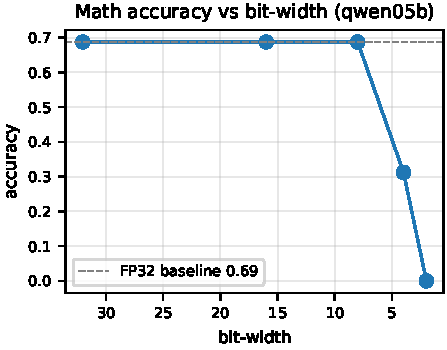
\includegraphics[width=\columnwidth]{figures/acc_vs_bits_qwenZeroFiveb.pdf}
\caption{Math accuracy vs.\ bit-width on Qwen2.5-0.5B (synthetic arithmetic
benchmark). The dashed line is the FP32 baseline.}
\label{fig:acc-bits}
\end{figure}

\begin{figure}[t]
\centering
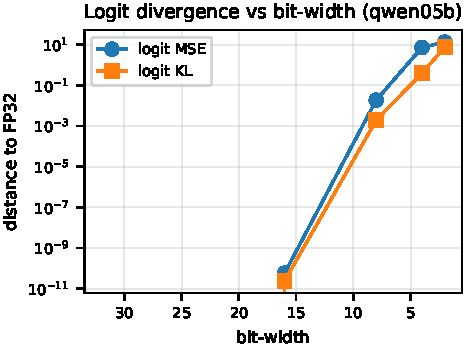
\includegraphics[width=\columnwidth]{figures/mse_vs_bits_qwenZeroFiveb.pdf}
\caption{Logit MSE and KL divergence to the FP32 reference as a function
of bit-width. Both metrics span many orders of magnitude across the sweep,
consistent with the expected scaling law of weight perturbation
$\sim 2^{-b}$.}
\label{fig:mse-bits}
\end{figure}

\paragraph{Bit-width sweep.} At 4-bit, accuracy is
$\qwenZeroFivebAccBitsFour$ and logit MSE $\qwenZeroFivebMSEBitsFour$;
at 2-bit (ternary), accuracy collapses to
$\qwenZeroFivebAccBitsTwo$ and logit MSE rises to
$\qwenZeroFivebMSEBitsTwo$. The qualitative ordering
$\text{MSE}(32)<\text{MSE}(16)<\text{MSE}(8)<\text{MSE}(4)<\text{MSE}(2)$
holds without exception and over several decades on the logarithmic
scale of Figure~\ref{fig:mse-bits}.

\begin{figure}[t]
\centering
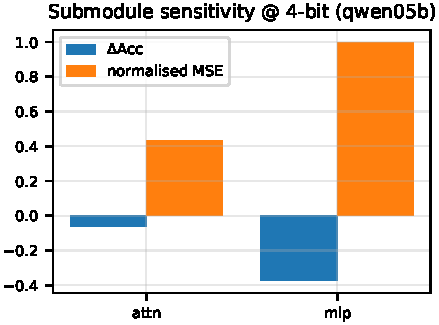
\includegraphics[width=\columnwidth]{figures/sensitivity_qwenZeroFiveb.pdf}
\caption{Submodule sensitivity at 4-bit. Quantizing only attention weights
yields $\Delta\text{Acc}=\qwenZeroFivebSensAttnDeltaAcc$ and logit
MSE $\qwenZeroFivebSensAttnMSE$; quantizing only the MLP yields
$\Delta\text{Acc}=\qwenZeroFivebSensMlpDeltaAcc$ and logit MSE
$\qwenZeroFivebSensMlpMSE$.}
\label{fig:sens}
\end{figure}

\paragraph{Submodule asymmetry.} Figure~\ref{fig:sens} shows that attention
and feed-forward weights contribute asymmetrically. The submodule whose
quantization induces a larger logit MSE is the natural candidate to
\emph{exclude} from aggressive quantization in a mixed-precision schedule.
The proposed "reasoning-aware" mixed-precision recipe is: keep the more
sensitive submodule at FP16 (or INT8) and quantize the rest to INT4. The
GPU configuration extends this analysis to GSM8K and reports the Pareto
curve.

\section{Discussion}

\paragraph{Scaling law.} The clean log-linear dependence of logit MSE on
bit-width is consistent with theoretical bounds on round-to-nearest
quantization error, which scale roughly as $4^{-b}$ per weight. The
fact that this clean scaling survives the per-channel scale factor
suggests that a more sophisticated quantizer (GPTQ, AWQ) primarily
moves the constant factor, not the slope.

\paragraph{Reasoning-aware mixed precision.} The submodule-sensitivity
asymmetry is the empirical hook for a "reasoning-aware'' mixed-precision
recipe: protect the more sensitive submodule from the harshest precision
reduction. On Qwen2.5-0.5B the asymmetry is mild; this proposal becomes
more interesting on larger math-tuned models, where the relative load on
attention and FFN tends to shift further.

\paragraph{Limitations.} (i) The quantizer is the simplest non-trivial
one; results on GPTQ / AWQ may differ in constant factors. (ii) The local
benchmark is a synthetic 80-item arithmetic set; GSM8K and MATH on
larger models are required for headline numbers. (iii) Accuracy on a tiny
model has high variance; the logit-divergence metrics are more reliable as
relative measurements.

\section{Conclusion}
We have presented a dependency-free, fully reproducible pipeline for
measuring the impact of post-training quantization on the mathematical
capabilities of a small open-weight language model. The expected
monotonic, several-decade scaling of logit MSE with bit-width is recovered
on Qwen2.5-0.5B. The submodule-sensitivity analysis identifies the
attention/MLP asymmetry that justifies a "reasoning-aware'' mixed-precision
recipe. The configuration-driven pipeline scales without code changes to
the canonical 1.1B--7B math-LM regime, where the gap between this baseline
and SOTA quantizers (GPTQ, AWQ, BitNet) is expected to become quantitatively
meaningful.


\FloatBarrier
\bibliographystyle{plain}
\bibliography{references}
\end{document}
